\documentclass{article}
\usepackage[utf8]{inputenc}
\usepackage{amsmath, amssymb, amsthm}
\usepackage{float}

\usepackage{listings}
\usepackage{xcolor}

\usepackage{tikz}
\usepackage{float}

\theoremstyle{definition}
\newtheorem{rules}{Rule}[section]
\newtheorem{definition}[rules]{Definition}
\newtheorem{remark}[rules]{Remark}
\newtheorem{example}[rules]{Example}

\definecolor{codegreen}{rgb}{0,0.6,0}
\definecolor{codegray}{rgb}{0.5,0.5,0.5}
\definecolor{codepurple}{rgb}{0.58,0,0.82}
\definecolor{backcolour}{rgb}{0.95,0.95,0.92}

\lstdefinestyle{thestyle}{
    backgroundcolor=\color{backcolour},
    basicstyle=\ttfamily\footnotesize,
    keywordstyle=\color{red!80}\bfseries,
    ndkeywordstyle=\color{blue!80}\bfseries,
    identifierstyle=\color{black},
    commentstyle=\color{codegreen},
    stringstyle=\color{codepurple},
    breakatwhitespace=false,
    breaklines=true,
    captionpos=b,
    keepspaces=true,
    numberstyle=\tiny\color{codegray},
    numbers=left,
    numbersep=2pt,
    showspaces=false,
    showstringspaces=false,
    showtabs=false,          
    tabsize=2
}

\lstset{style=thestyle}

\lstdefinelanguage{TML}{ 
    keywords={changeto, move, goto, if, switch, while, module, accept, reject, halt, alphabet},
    ndkeywords={left, right, tapehead, blank},
    sensitive=true,
    comment=[l]{//},
    morecomment=[s]{/*}{*/},
    morestring=[b]',
    morestring=[b]"
}

\title{TML Specification}
\author{Pete Gautam}

\begin{document}
    \maketitle
    \begin{abstract}
        This document contains the specification of the TM programming language (called Turing Machine Language, or TML), and how it can be used to change the state of a tape. In the first section, we discuss TML rules (the EBNF and contextual rules), and give examples of valid and invalid TML programs. In the second section, we define tapes and how a TML program can be executed on a tape. This section also includes some examples of executing a TM program on a given tape.
    \end{abstract}

    \section{TML rules}
    In this section, we define the rules that a valid program in TML should obey. First, the following is the specification of the TML in EBNF:
    \begin{align*}
        \textit{program} &= \textit{alphabet} \ \textit{module}^+ \\
        \textit{alphabet} &= \texttt{alphabet} \ \texttt{=} \ \texttt{\{} \ \textit{seq-val} \ \texttt{\}} \\
        \textit{module} &= \texttt{module} \ \textit{id} \ \texttt{\{} \ \textit{block}^+ \ \texttt{\}} \\
        \textit{block} &= \textit{basic-block} \ | \ \textit{switch-block} \\
        \textit{switch-block} &= \texttt{switch tapehead \{} \ \textit{case-block}^+ \ \texttt{\}} \\
        \textit{case-block} &= \textit{if-block} \ | \ \textit{while-block} \\
        \textit{if-block} &= \texttt{if} \ \textit{seq-val} \ \texttt{\{} \textit{block}^+ \texttt{\}} \\
        \textit{while-block} &= \texttt{while} \ \textit{seq-val} \ \texttt{\{} \ \textit{core-com}^+ \ \texttt{\}} \\
        \textit{basic-block} &= (\textit{core-com} \ | \ \textit{flow-com})^+ \\
        \textit{core-com} &= \texttt{move} \ \textit{direction} \ | \ \texttt{changeto} \ \textit{value} \\
        \textit{flow-com} &= \texttt{goto} \ \textit{id} \ | \ \textit{terminate} \\
        \textit{terminate} &= \texttt{reject} \ | \ \texttt{accept} \\
        \textit{direction} &= \texttt{left} \ | \ \texttt{right} \\
        \textit{seq-val} &= (\textit{value}^* \texttt{,}) \ \textit{value} \\
        \textit{value} &= \texttt{blank} \ | \ \texttt{a} \ | \ \texttt{b} \ | \ \texttt{c} \ | \ \dots \ | \ \texttt{z} \ | \ \texttt{0} \ | \ \texttt{1} \ | \ \dots \ | \ \texttt{9} \\
        \textit{id} &= (\texttt{a} \ | \ \texttt{b} \ | \ \texttt{c} \ | \ \dots \ | \ \texttt{z} \ | \ \texttt{A} \ | \ \texttt{B} \ | \ \texttt{C} \ | \ \dots \ | \ \texttt{Z})^+
    \end{align*}
    
    Next, we analyse the rules of a TML program.
    \begin{rules}
        A valid TML program is composed of the \emph{alphabet}, followed by one or more \emph{modules}.
    \end{rules}
    \begin{rules}
        A module contains a collection of a \emph{blocks} (a specific sequence of commands). There are two types of blocks- \emph{basic blocks} and \emph{switch blocks}.
    \end{rules}
    \begin{rules}
        A basic block consists of \emph{basic commands} (\textit{changeto}, \textit{move} or \textit{flow} command). A basic block consists of at least one basic command, but it is not necessary for a basic block to be composed of all the basic commands. If multiple commands are present in a basic block, they must be in the following order- \textit{changeto}, \textit{move} and \textit{flow} command.
    \end{rules}
    \begin{example}
        The following is a simple TML program:
\begin{lstlisting}[language=TML]
alphabet = {"a", "b"}
module simple {
    changeto blank
    move right
    changeto a
    move left
    accept
}
\end{lstlisting}
    It is composed of a single module, called \texttt{simple}. The module has 2 basic blocks- lines 3-4, and lines 5-7.
    \end{example}
    \begin{remark}
        In the example above, we could have also said that there were 5 basic blocks, one in each line from line 3 to line 7. If it is possible for us to break a module into blocks in different ways, we always choose the one that ends up with the fewest number of blocks. In this case, we cannot have just one block since lines 3-5 do not form a basic block- there are two \textit{changeto} commands. So, we have 2 basic blocks above.
    \end{remark}
    
    \begin{rules}
        A \emph{switch block} consists of a single switch statement. A switch statement must contain precisely one case (\textit{if} or \textit{while} command) for each of the letter in the alphabet, including the \texttt{blank} letter. The first block of a case block must be a basic block.
    \end{rules}
    \begin{rules}
        The body of an \textit{if} command can be composed of multiple blocks. These blocks can be both basic blocks and switch blocks.
    \end{rules}
    \begin{rules}
        The body of a \textit{while} command must be composed of a single basic block. The basic block cannot have a \textit{flow} command. Further, a switch block must be the final block present; it cannot be followed by any other block, basic or switch.
    \end{rules}
    
    \begin{example}
        The following is another TML program:
\begin{lstlisting}[language=TML]
alphabet = {"0", "1"}
module isEven {
    switch tapehead {
        while 0, 1 {
            move right
        } if blank {
            move left
            switch tapehead {
                if 0 {
                    accept
                } if 1, blank {
                    reject
                }
            }
        }
    }
}
\end{lstlisting}
    It is composed of a single module \texttt{isEven}. The module has:
    \begin{itemize}
        \item a switch block at lines 3-16;
        \item a basic block at line 5;
        \item a basic block at line 7;
        \item a nested switch block at lines 8-14;
        \item a basic block at line 10; and
        \item a basic block at line 12.
    \end{itemize}
    \end{example}
    \newpage

    \section{TML execution}
    In this section, we discuss how a valid TML program can execute a tape. The tape we will be using has infinite spaces in both directions.
    \begin{definition}
        Let $\Sigma$ be an alphabet. A \emph{tape $T$ on $\Sigma$} is a function $T: \mathbb{Z} \to \Sigma^+$, where $\Sigma^+ = \Sigma \cup \{\texttt{blank}\}$.
    \end{definition}
    \begin{remark}
        A valid TML program always specifies the alphabet. This corresponds to the alphabet $\Sigma$ used in the tape.
    \end{remark}
    \noindent Although there are many possible tapes, we will only be interested in tapes that obey some rules.
    \begin{definition}
        Let $\Sigma$ be an alphabet and let $T$ be a tape on $\Sigma$. Then, $T$ is a \emph{valid tape} if only finitely many symbols on $T$ are not \texttt{blank}, and all the values that can be non-\texttt{blank} are non-\texttt{blank}. That is, there exist integers $a, b$ such that for all $x \in \mathbb{Z}$, $T(x)$ is not \texttt{blank} if and only $x \geq a$ and $x \leq b$.
    \end{definition}
    \begin{remark}
        In a valid tape, there are only finitely many values that are non-\texttt{blank} and there is no gap between any two non-\texttt{blank} values.
    \end{remark}
    \begin{remark}
        We require the tape to have finitely many non-\texttt{blank} entries so that we start execution with the tapehead at the first non-\texttt{blank} entry. Moreover, this ensures that going from the start of the tape to the end does not create an infinite loop- this is a very common procedure. If we allowed for infinitely many non-\texttt{blank} entries, we would need to specify where the initial location of the tapehead is. Moreover, there would be much fewer programs that we could write which are guaranteed to terminate.
    \end{remark}
    \begin{remark}
        A valid tape can always be represented as an illustration. For instance, consider the following valid tape $T$ on $\{0, 1\}$:
        \[T(x) = \begin{cases}
            0 & x \in \{1, 3, 4\} \\
            1 & x \in \{2\} \\
            \texttt{blank} & \text{otherwise}.
        \end{cases}\]
        Then, an illustration of the tape is:
        \begin{figure}[H]
            \centering
            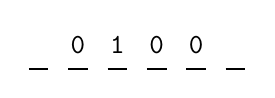
\begin{tikzpicture}
                \draw[thick] (-0.25, 0) -- (0, 0);
                \foreach \x[count=\i] in {0, 1, 0, 0} {
                    \draw[thick] (\i*0.5-0.25, 0) -- (\i*0.5, 0);
                    \node at (\i*0.5-0.125, 0.3) {\texttt{\x}};
                }
                \draw[thick] (2.25, 0) -- (2.5, 0);
            \end{tikzpicture}
            \caption{The tape as a diagram.}
        \end{figure}
        \noindent Only the non-\texttt{blank} values are represented. Blank ones are represented by empty lines.
    \end{remark}
    \begin{remark}
        More than one tape definition can result in the same diagram. In the case above, the following tape $S$ on $\{0, 1\}$ also has the same diagram.
        \[S(x) = \begin{cases}
            0 & x \in \{0, 2, 3\} \\
            1 & x \in \{1\} \\
            \texttt{blank} & \text{otherwise}.
        \end{cases}\]        
    \end{remark}
    \begin{example}
Consider the following TML program:
\begin{lstlisting}[language=TML]
alphabet = {"a", "b"}
module isSecondValueA {
    move right
    switch tapehead {
        if a {
            accept
        } if b, blank {
            reject
        }
    }
}
\end{lstlisting}
    The following is a valid tape for the program:
    \begin{figure}[H]
        \centering
        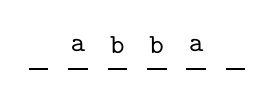
\begin{tikzpicture}
            \draw[thick] (-0.25, 0) -- (0, 0);
            \foreach \x[count=\i] in {a, b, b, a} {
                \draw[thick] (\i*0.5-0.25, 0) -- (\i*0.5, 0);
                \node at (\i*0.5-0.125, 0.3) {\texttt{\x}};
            }
            \draw[thick] (0.5*5-0.25, 0) -- (0.5*5, 0);
        \end{tikzpicture}
    \end{figure}
    \end{example}

    Now, we will define how we can execute a TML program on a valid tape.
    \begin{definition}
        Let $P$ be a TML program, let $T$ be a valid tape for the program with $i$ the smallest integer such that $T(i)$ is not \texttt{blank} ($i$ is the initial \emph{tapehead index} and $T(i)$ the initial \textit{tapehead value}). We \emph{execute $P$ on $T$} by constructing (countable) different tapes until execution is terminated. We first take the given tape and the tapehead index and execute it using the first block $b$ in the first module of $P$ to construct the next tape $T'$ and next tapehead index $i'$. This is done as follows:
        \begin{itemize}
            \item if the block is a switch block, we take the first block from the case corresponding to the tapehead value- now, we must have a basic block;
            \item if there is a \textit{changeto} \texttt{val} command in the basic block, the next tape $T'$ is given by 
            \[T'(x) = \begin{cases}
                \texttt{val} & x = i \\
                T(x) & \text{otherwise}.
            \end{cases}\]
            If the \textit{changeto} command is missing, then the tapehead $T' = T$.
            \item if there is a \textit{move} \texttt{dir} command in the basic block, the next tapehead index is given by:
            \[i' = \begin{cases}
                i+1 & \texttt{dir} = \texttt{right} \\
                i-1 & \texttt{dir} = \texttt{left}.
            \end{cases}\]
            If the \textit{move} command is missing, then $i' = i-1$.
            \item we either terminate or determine the next block $b'$ to execute (in decreasing precedence):
            \begin{itemize}
                \item if the block is the body of a while case block, then $b' = b$, i.e. we execute this switch block again (not necessarily the same case block); 
                \item if the block contains a terminating \textit{flow} command, we terminate and return the terminated state;
                \item if the block contains a \textit{goto} \texttt{mod} command, then $b'$ is the first block of the module \texttt{mod};
                \item if the block is not the final block in the module, then $b'$ is next block in this module;
                \item otherwise, we terminate and return the state \texttt{reject}.
            \end{itemize}
        \end{itemize}
        If execution is not terminated, we execute the block $b'$ with the new tape $T'$ and a new tapehead index $i'$.
    \end{definition}
    \begin{remark}
        By construction, for a valid program, precisely one of the 5 possible step applies when choosing the next block to execute or terminate.
    \end{remark}
    
    \begin{example}
        Consider the following TML program:
\begin{lstlisting}[language=TML]
alphabet = {"a", "b"}
module palindrome {
    switch tapehead {
        if blank {
            accept
        } if a {
            changeto blank
            move right
            switch tapehead {
                while a, b {
                    move right
                } if blank {
                    move left
                    switch tapehead {
                        if blank, a {
                            changeto blank
                            move left
                            goto restart
                        } if b {
                            reject
                        }
                    }
                }
            }
        }  if b {
            changeto blank
            move right
            switch tapehead {
                while a, b {
                    move right
                } if blank {
                    move left
                    switch tapehead {
                        if blank, b {
                            changeto blank
                            move left
                            goto restart
                        } if a {
                            reject
                        }
                    }
                }
            }
        }
    }
}
module restart {
    switch tapehead {
        while a, b {
            move left
        } if blank {
            move right
            goto palindrome
        }
    }
}
\end{lstlisting}
    We will execute the program on the following tape.
    \begin{figure}[H]
        \centering
        \begin{tikzpicture}
            \draw[thick] (-0.25, 0) -- (0, 0);
            \foreach \x[count=\i] in {a, b, a} {
                \draw[thick] (\i*0.5-0.25, 0) -- (\i*0.5, 0);
                \node at (\i*0.5-0.125, 0.3) {\texttt{\x}};
            }
            \draw[thick] (1.75, 0) -- (2, 0);
    
            \draw[->, thick] (0.375, -0.5) -- (0.375, -0.1);
        \end{tikzpicture}
    \end{figure}
    \noindent The arrow points to the tapehead value. We first execute the switch block at \texttt{palindrome}. Since the tapehead value is \texttt{a}, we execute the basic block at lines 7-8. So, we change the tapehead value to \texttt{blank}, and the tapehead moves to the right by one step. Since this is an \textit{if}-block, without a flow command, and there is a block following this one, the next block to be executed is the switch block at lines 9-24. Now, the current tape is the following.
    \begin{figure}[H]
        \centering
        \begin{tikzpicture}
            \draw[thick] (-0.25, 0) -- (0, 0);
            \foreach \x[count=\i] in {b, a} {
                \draw[thick] (\i*0.5-0.25, 0) -- (\i*0.5, 0);
                \node at (\i*0.5-0.125, 0.3) {\texttt{\x}};
            }
            \draw[thick] (1.25, 0) -- (1.5, 0);
    
            \draw[->, thick] (0.375, -0.5) -- (0.375, -0.1);
        \end{tikzpicture}
    \end{figure}
    \noindent The current block is a switch block. The tapehead value is \texttt{b}, so we are at the \textit{while} command at line 11. The basic block here only contains a \textit{move} command. So, we leave the tape as is, and the tapehead moves to the right once. This is a \textit{while} command, so the next block to execute is still this switch block. The current tape state is the following.
    \begin{figure}[H]
        \centering
        \begin{tikzpicture}
            \draw[thick] (-0.25, 0) -- (0, 0);
            \foreach \x[count=\i] in {b, a} {
                \draw[thick] (\i*0.5-0.25, 0) -- (\i*0.5, 0);
                \node at (\i*0.5-0.125, 0.3) {\texttt{\x}};
            }
            \draw[thick] (1.25, 0) -- (1.5, 0);
    
            \draw[->, thick] (0.875, -0.5) -- (0.875, -0.1);
        \end{tikzpicture}
    \end{figure}
    \noindent The current block is still a switch block. The tapehead value is \texttt{a}, so we execute the same \textit{while} command at line 11. Moreover, the next block to execute is still the switch block. Now, the current tape state is the following.
    \begin{figure}[H]
        \centering
        \begin{tikzpicture}
            \draw[thick] (-0.25, 0) -- (0, 0);
            \foreach \x[count=\i] in {b, a} {
                \draw[thick] (\i*0.5-0.25, 0) -- (\i*0.5, 0);
                \node at (\i*0.5-0.125, 0.3) {\texttt{\x}};
            }
            \draw[thick] (1.25, 0) -- (1.5, 0);
    
            \draw[->, thick] (1.375, -0.5) -- (1.375, -0.1);
        \end{tikzpicture}
    \end{figure}
    \noindent For the third time, we are executing the same switch block. Now, however, the tapehead value is \texttt{blank}, so we execute the first block of the \textit{if} command at line 13. Since this is an \textit{if} command and this is not the last block in the if command, the next block to execute is the switch block at lines 14-22.
    \begin{figure}[H]
        \centering
        \begin{tikzpicture}
            \draw[thick] (-0.25, 0) -- (0, 0);
            \foreach \x[count=\i] in {b, a} {
                \draw[thick] (\i*0.5-0.25, 0) -- (\i*0.5, 0);
                \node at (\i*0.5-0.125, 0.3) {\texttt{\x}};
            }
            \draw[thick] (1.25, 0) -- (1.5, 0);
    
            \draw[->, thick] (0.875, -0.5) -- (0.875, -0.1);
        \end{tikzpicture}
    \end{figure}
    \noindent Now, the current block is a switch block. The tapehead value is \texttt{a}, so we take the basic block at lines 16-18. The value of the tapehead becomes \texttt{blank}, and the tapehead moves to the left. The next block to execute is the switch block in \texttt{restart}.
    \begin{figure}[H]
        \centering
        \begin{tikzpicture}
            \draw[thick] (-0.25, 0) -- (0, 0);
            \foreach \x[count=\i] in {b} {
                \draw[thick] (\i*0.5-0.25, 0) -- (\i*0.5, 0);
                \node at (\i*0.5-0.125, 0.3) {\texttt{\x}};
            }
            \draw[thick] (0.75, 0) -- (1, 0);
    
            \draw[->, thick] (0.375, -0.5) -- (0.375, -0.1);
        \end{tikzpicture}
    \end{figure}
    \noindent Since the current tapehead value is \texttt{b}, we execute the basic block at line 50. So, we move to the left, and the tape is left as is. Moreover, since this is a while block, the next block to execute is still the switch block.
    \begin{figure}[H]
        \centering
        \begin{tikzpicture}
            \draw[thick] (-0.25, 0) -- (0, 0);
            \foreach \x[count=\i] in {b} {
                \draw[thick] (\i*0.5-0.25, 0) -- (\i*0.5, 0);
                \node at (\i*0.5-0.125, 0.3) {\texttt{\x}};
            }
            \draw[thick] (0.75, 0) -- (1, 0);
    
            \draw[->, thick] (-0.125, -0.5) -- (-0.125, -0.1);
        \end{tikzpicture}
    \end{figure}
    \noindent Since the current tapehead state is \texttt{blank}, we execute the basic block at lines 52-53. So, we move to the right, and the tape is left as is. The next block to execute is the switch block at \texttt{palindrome}.
    \begin{figure}[H]
        \centering
        \begin{tikzpicture}
            \draw[thick] (-0.25, 0) -- (0, 0);
            \foreach \x[count=\i] in {b} {
                \draw[thick] (\i*0.5-0.25, 0) -- (\i*0.5, 0);
                \node at (\i*0.5-0.125, 0.3) {\texttt{\x}};
            }
            \draw[thick] (0.75, 0) -- (1, 0);
    
            \draw[->, thick] (0.375, -0.5) -- (0.375, -0.1);
        \end{tikzpicture}
    \end{figure}
    \noindent Since the current tapehead state is \texttt{b}, we execute the basic block at lines 26-27. So, we change the tapehead value to \texttt{blank}, move to the right. This is a while block, so the next block to be executed is still the switch block.
    \begin{figure}[H]
        \centering
        \begin{tikzpicture}
            \draw[thick] (-0.25, 0) -- (0, 0);
            \draw[thick] (0.25, 0) -- (0.5, 0);
            \draw[thick] (0.75, 0) -- (1, 0);
    
            \draw[->, thick] (0.875, -0.5) -- (0.875, -0.1);
        \end{tikzpicture}
    \end{figure}
    \noindent The current tapehead state is \texttt{blank}, so we execute the basic block at line 32. We move to the left and keep the tape as is. The next block to execute is the switch block at lines 33-41.
    \begin{figure}[H]
        \centering
        \begin{tikzpicture}
            \draw[thick] (-0.25, 0) -- (0, 0);
            \draw[thick] (0.25, 0) -- (0.5, 0);
            \draw[thick] (0.75, 0) -- (1, 0);
    
            \draw[->, thick] (0.375, -0.5) -- (0.375, -0.1);
        \end{tikzpicture}
    \end{figure}
    \noindent The current tapehead value is \texttt{blank}, so we execute the basic block at lines 35-37. We keep the tape as is, and move to the left. The next block to execute is the switch block at lines 48-55.
    \begin{figure}[H]
        \centering
        \begin{tikzpicture}
            \draw[thick] (-0.25, 0) -- (0, 0);
            \draw[thick] (0.25, 0) -- (0.5, 0);
            \draw[thick] (0.75, 0) -- (1, 0);
    
            \draw[->, thick] (-0.125, -0.5) -- (-0.125, -0.1);
        \end{tikzpicture}
    \end{figure}
    \noindent The current tapehead value is \texttt{blank}, so we execute the basic block at lines 52-53. In that case, we move to the right and go to the switch block at \texttt{palindrome}.
    \begin{figure}[H]
        \centering
        \begin{tikzpicture}
            \draw[thick] (-0.25, 0) -- (0, 0);
            \draw[thick] (0.25, 0) -- (0.5, 0);
            \draw[thick] (0.75, 0) -- (1, 0);
    
            \draw[->, thick] (0.375, -0.5) -- (0.375, -0.1);
        \end{tikzpicture}
    \end{figure}
    \noindent The current tapehead value is \texttt{blank}, so we execute the basic block at line 5. We move to the left, keep the tapehead as is, and accept the tape. In that case, the final state of the tape is the following.
    \begin{figure}[H]
        \centering
        \begin{tikzpicture}
            \draw[thick] (-0.25, 0) -- (0, 0);
            \draw[thick] (0.25, 0) -- (0.5, 0);
            \draw[thick] (0.75, 0) -- (1, 0);
    
            \draw[->, thick] (-0.125, -0.5) -- (-0.125, -0.1);
        \end{tikzpicture}
    \end{figure}
\end{example}
\end{document}
